\documentclass[11pt]{article}

% set these commands
\newcommand{\course}{CSCI 534}
\newcommand{\proj}{Homework 05}
\newcommand{\dueDate}{3-25-2021}
\newcommand{\instructor}{David L. Millman}

\usepackage{../macros}

\begin{document}

\coverpage{05}

\newpage
\section*{Problem 1}

In Homework 1, we considered a plane-sweep algorithm for determining whether
there is any intersection among a collection of $n$ circles in the plane. Here
we consider a variant of this problem. The input consists of a collection of $n$
closed circular disks, all having the same radius. (Via scaling, we may assume
that they are all unit disks.) Let $C = \{c_1, \ldots , c_n\}$ denote the center
points of these disks, and let $\{D_1, \ldots, D_n\}$ denote the actual disks.
Thus, $D_i$ consists of the points that lie within unit distance of $c_i$. Let
$U = D_1 \cup \ldots \cup D_n$ denote the union of these disks. The boundary of
$U$ may generally consist of multiple parts, each of which consists of a cycle
of circular arcs connected by vertices. (In Fig. 4 the boundary consists of
three cycles. The vertices are shown as white dots).

\begin{figure}[h]
    \centering
    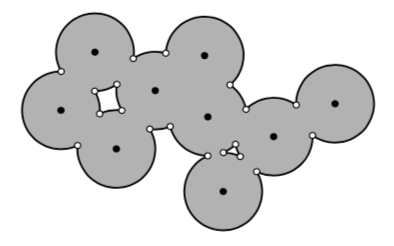
\includegraphics[width=0.4\textwidth]{union-of-disks}
    \caption{Problem 4: Union of disks}
\end{figure}


\begin{enumerate}

    \item Present an algorithm that reports all the vertices on the boundary of
        $U$. (Note that circle intersection points in the interior of the union
        are explicitly excluded.) Your algorithm should run in time $O(n \log
        n)$.  The order in which the vertices are output is arbitrary. (Hint:
        Don't try to modify the algorithm from Homework 2. A different approach
        is needed.... think giraffes)

    \item Prove that the number of vertices reported by your algorithm is
        $O(n)$.

\end{enumerate}

\newpage
\section*{Problem 2}

Suppose we are given a subdivision of the plane into $n$ convex regions. We
suspect that this subdivision is a Voronoi diagram, but we do not know the
sites. Develop an algorithm that finds a set of $n$ point sites whose Voronoi
diagram is exactly the given subdivision, if such a set exists. \\\\

\answer
So we are given a subdivision of the plane into convex regions and we wish to report a set of $n$ sites whose Voronoi diagram is the subdivision (if it possible).
Let's consider two trivial cases before giving an algorithm.
If $n=1$, then any point works and if $n=2$ we can just take any point not on the edge of the subdivision and its reflection.
From here on out, we will assume $n > 2$.
For general position, we will assume that no vertex in the subdivision has degree higher than 3.

Label the subdivsion $D$.
Suppose for some face in $D$, we have a single point $p$ that must be the site of the face (if $D$ is a Voronoi diagram).
Assume that the faces of $D$ are labeled $1, 2, \ldots, n$.
We will prove that we can compute that point $p$ later in the problem.

Here is a quick prose description of the algoritm.
We take $D$ to be a DCEL, $p$ is the site we know must exist, and $k$ is the label for the face that $p$ belongs to.
We are going to start at $p$ and reflect it across each edge of the face $k$.
If $p$ is a site in a voronio diagram, its reflection across an edge must also be a site.
We record every reflected point in an array and add faces to a processing queue as we come across them (note each face can only be added once).
If we ever find that a newly reflected point conflicts with a point already found in that face, we know that the subdivision is not a voronoi diagram.
We now present the algorithm.

\begin{algorithm}
\caption{Computing the Voronoi Sites}
\label{alg:voronoisites}
    \begin{algorithmic}[1]
    \Function{VoronoiSites}{$D$, $p = (p_x, p_y)$, $k$}
        \State S $\gets [$null, $\ldots, $ null$]$ // empty array of size $n$
        \State S[$k$] $\gets p$
        \State queue $\gets [ k ]$  // a queue for face labels
        \While{queue is not empty}
            \State $i \gets$ pop the queue
            \For{every edge $e$ of face i}
                \State $j \gets $ label of the face across $e$
                \State $q \gets $ reflection of the point S[$i$] across $e$
                \If{S[$j$] $=$ null}
                    \State S[$j$] $\gets q$
                    \State add $j$ to the queue
                \Else{ {\bf if} S[$j$] $\neq q$}
                    \State \Return NOT VORONOI
                \EndIf
            \EndFor
        \EndWhile
        \State \Return $S$
    \EndFunction
    \end{algorithmic}
\end{algorithm}

\begin{figure}[h]
    \centering
    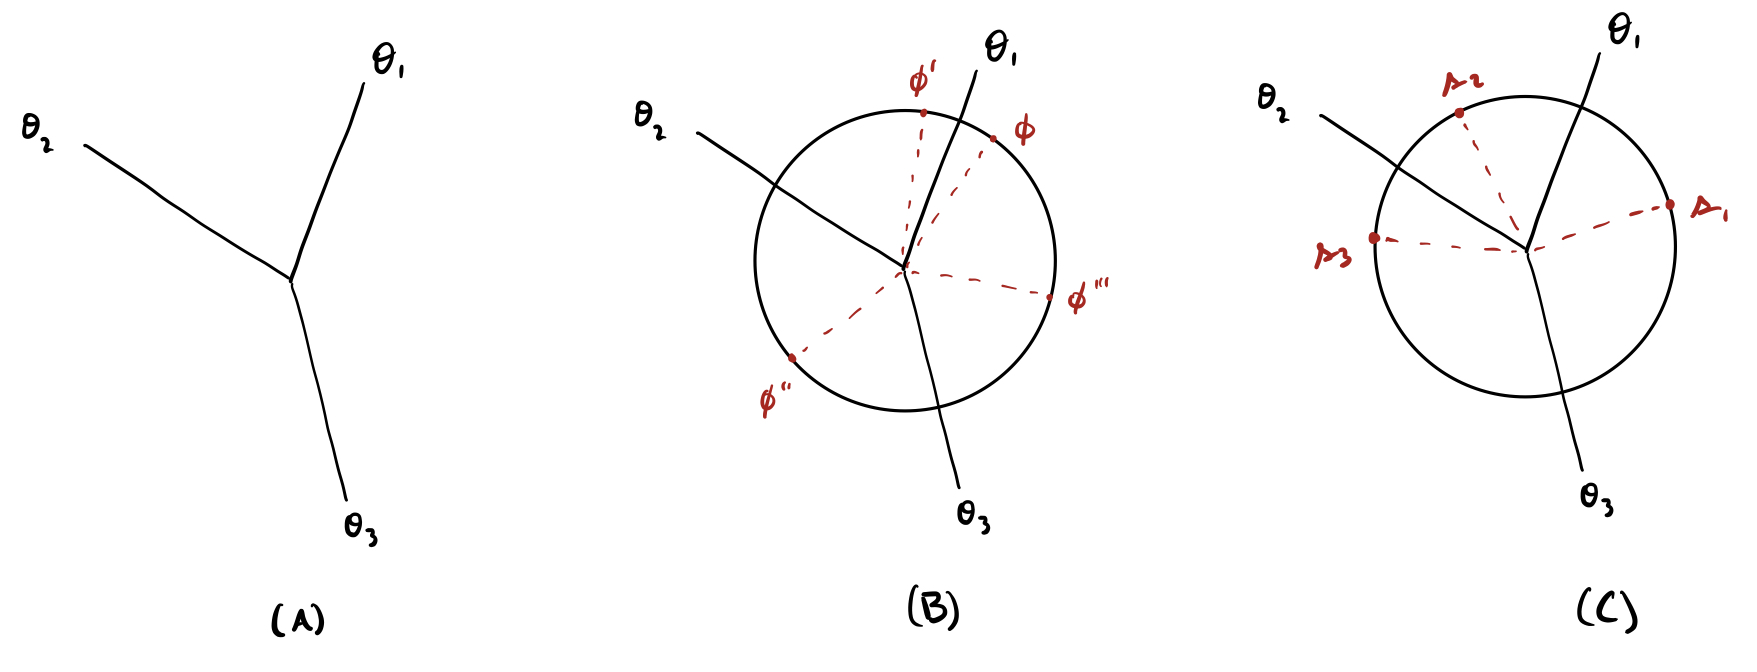
\includegraphics[width=0.9\textwidth]{solvingphi}
    \label{fig:solvingphi}
    \caption{Solving for $\phi$}
\end{figure}

\begin{figure}[h]
    \centering
    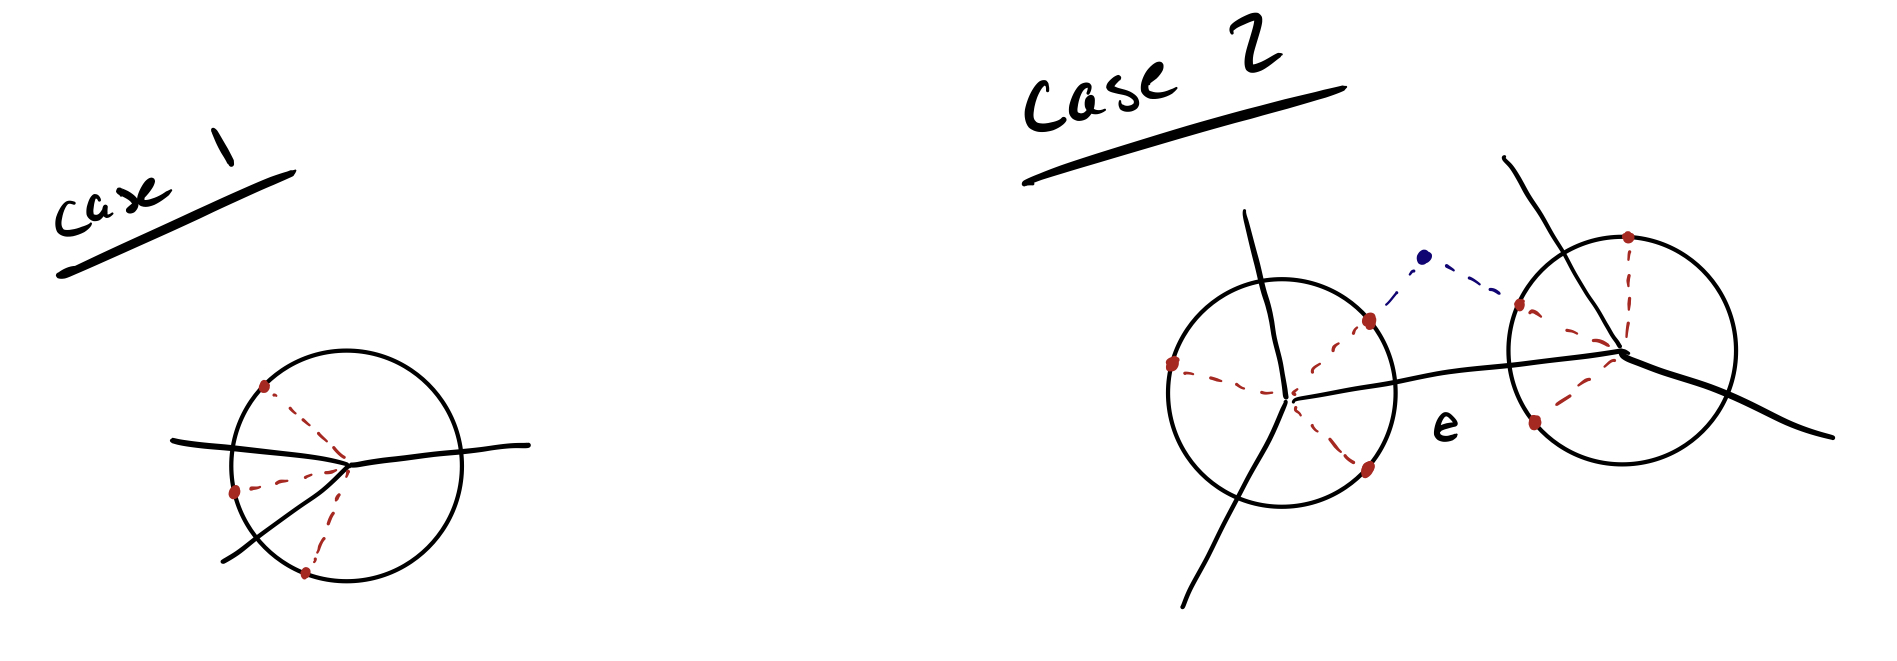
\includegraphics[width=0.6\textwidth]{site}
    \label{fig:site}
    \caption{Computing the site}
\end{figure}

\end{document}
